\section{Durchführung}
\label{sec:Durchführung}
\begin{figure}
    \centering
    \caption{Der Aufbau des Versuchs.}
    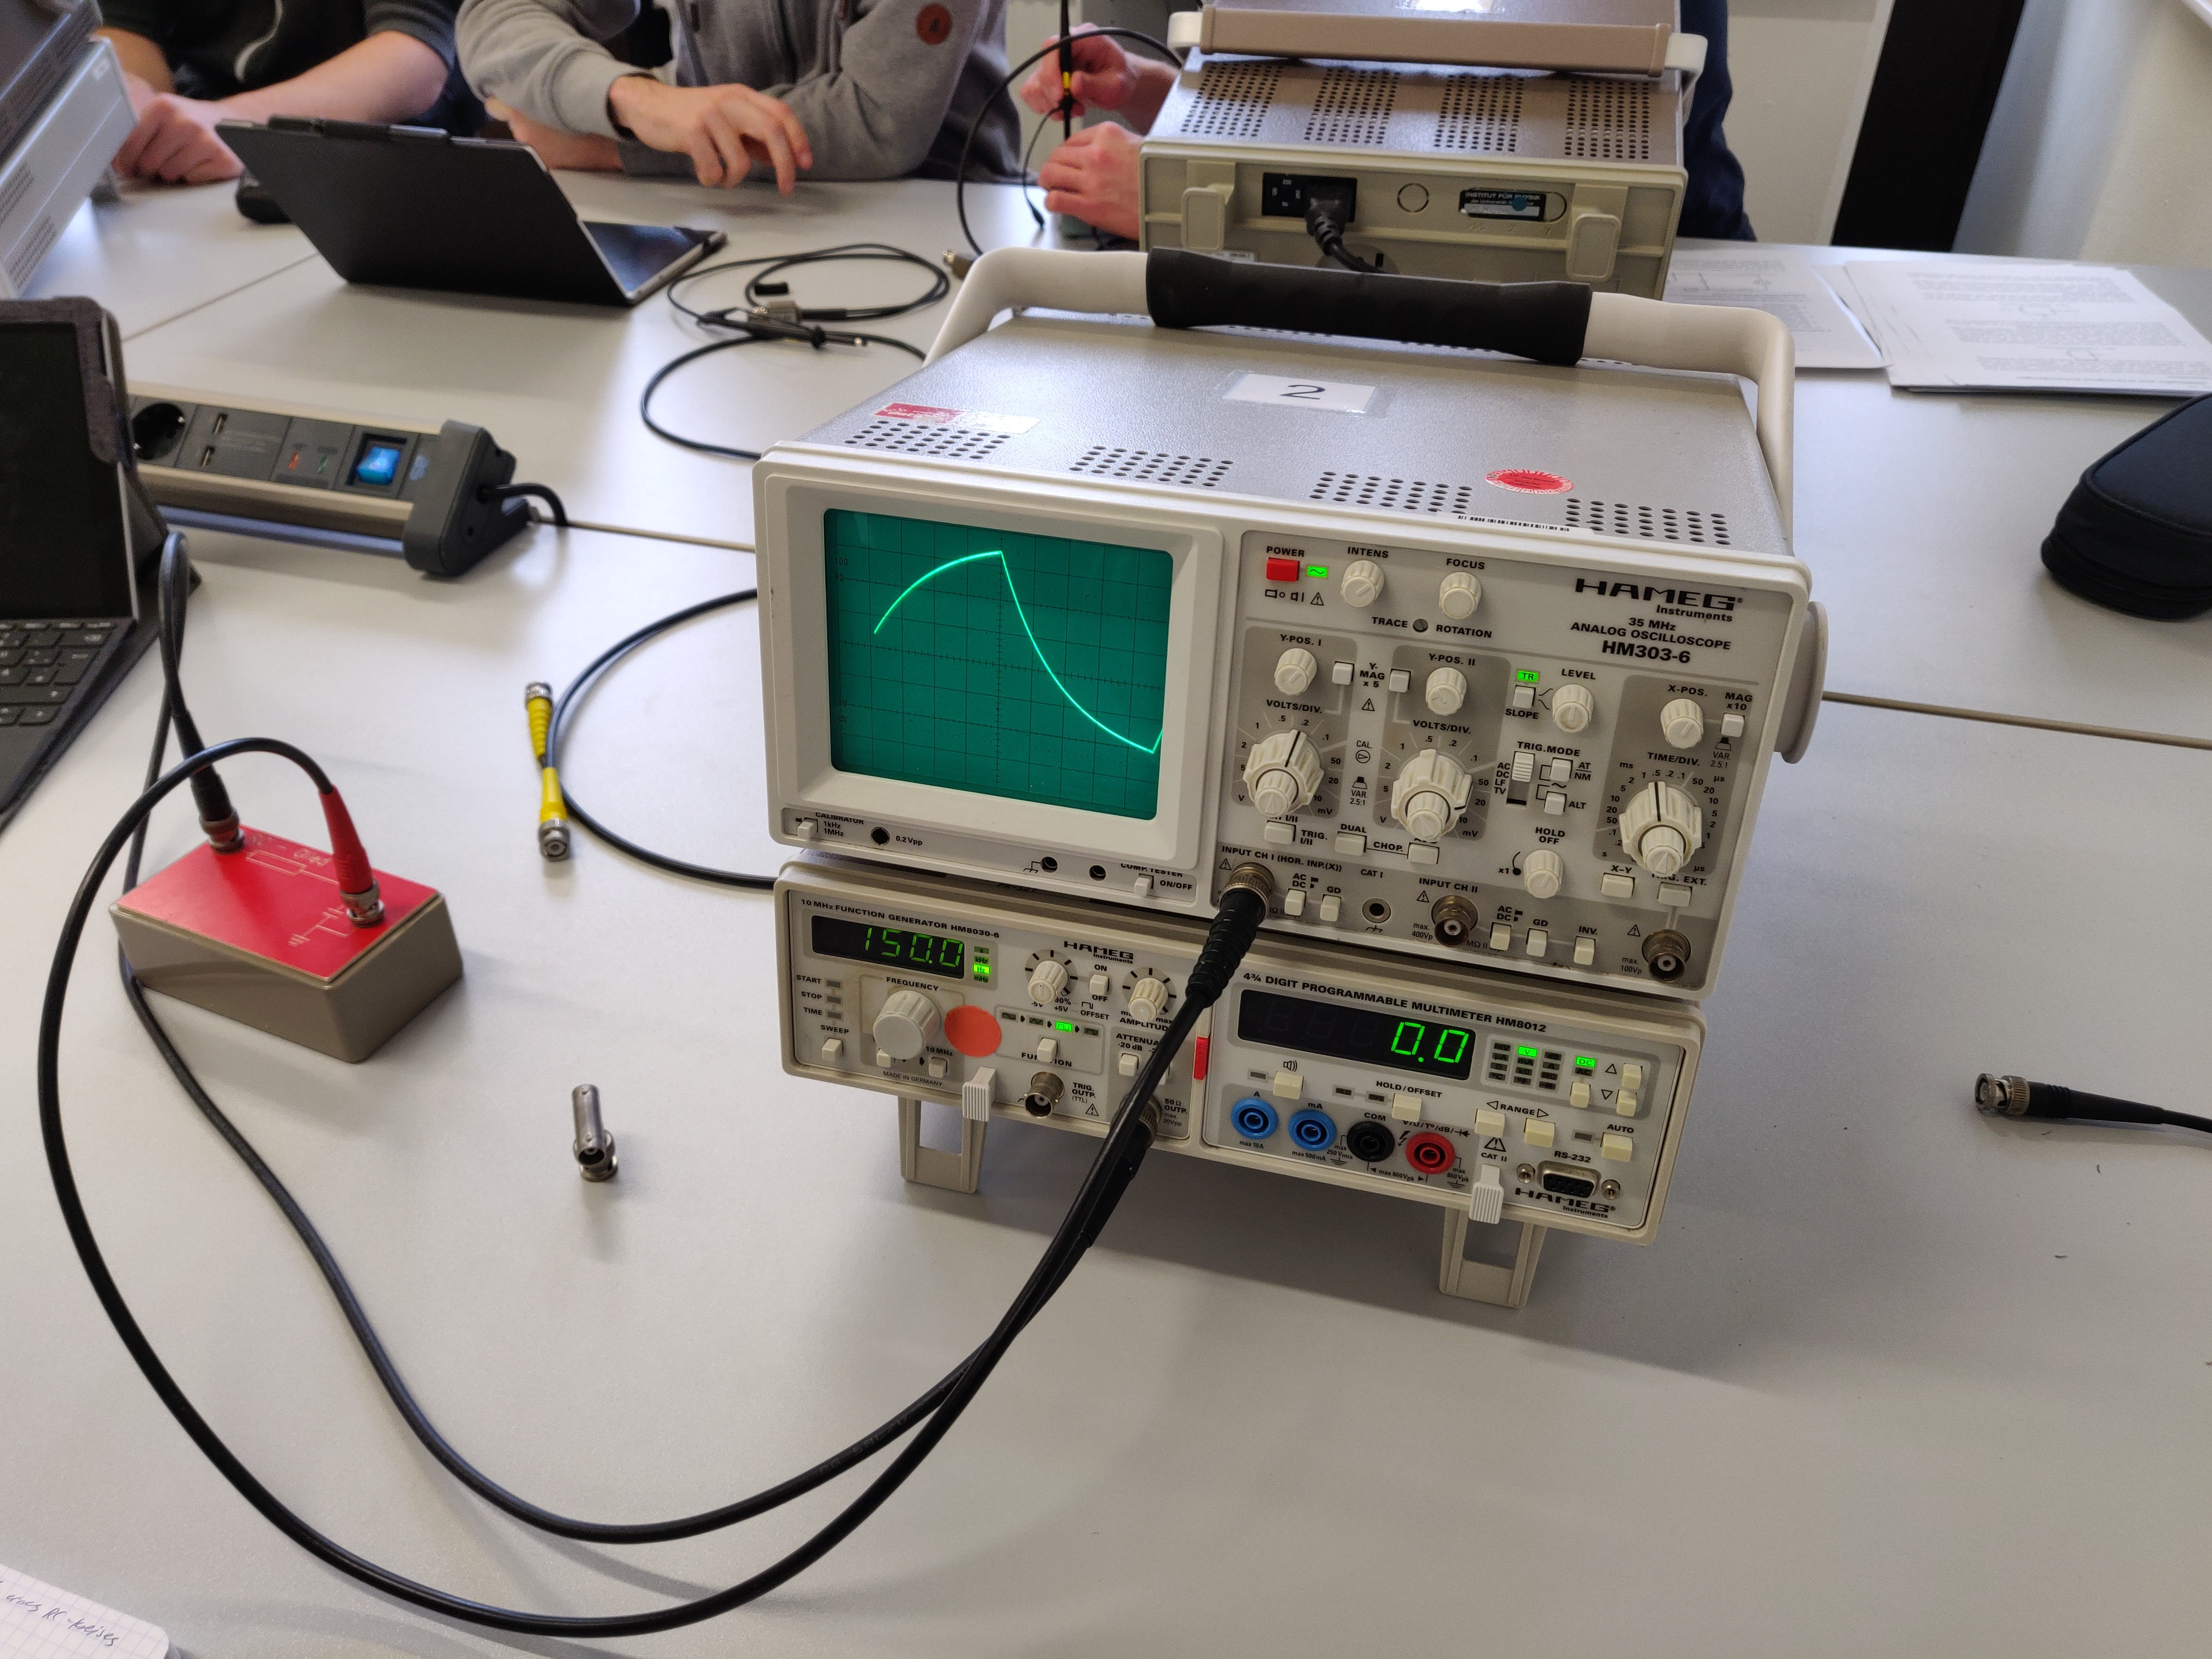
\includegraphics[width=\textwidth]{content/data/IMG_20191203_122746.jpg}
    \label{fig:aufbau}
\end{figure}

\subsection{Entladung des RC-Kreises}
\label{sec:1}
Der Versuch wird wie in Abbildung \ref{fig:aufbau} aufgebaut.
Der RC-Kreis wird zunächst an einem Wechselspannungsgenerator angeschlossen.
Der Spannungsgenerator erzeugt eine Rechteck Spannung.
Dabei wird am Kondensator mithilfe eines Oszilloskops die Spannung ziwschen den beiden Platten gemessen.
Nun wird die Spannung des Wechselspannungsgenerator auf einen festen Wert eingestellt und notiert.
Daraufhin muss das Oszilloskop so eingestellt werden, dass eine stehendes Bild zu sehen ist, in diesem Fall soll das Bild einen Entladevorgang zeigen.
Nun werden zwölf Werte in regelmäßigen Abständen vom Oszilloskop abgelesen und notiert, die später zur Auswertung genutzt werden.
\FloatBarrier
\subsection{Frequenzabhängigkeit des RC-Kreises}

\begin{figure}
    \centering
    \caption{Veranschaulichung der aufgenommen Werte \cite[S.282]{anleitung}.}
    \includegraphics[width=\textwidth]{content/data/a_und_b.jpg}
    \label{fig:a_und_b}
\end{figure}

Der Aufbau wird wie in Teil \ref{sec:1} erklärt beibehalten.
Nun wird allerdings am Spannungsgenerator eine Sinusspannung erzeugt, dessen Frequenz im laufe des Versuch variiert wird.
Da bei diesem Teil des Versuch der Phasenunterschied und die Amplitude der Spannung am Kondensator und am Generator untersucht werden soll, wird auch der Generator am Oszilloskop angeschlossen.
Dadurch sind beide Spannungen zu sehen.
Nun wird eine Wechselspannung mit niedriger Frequenz am Generator eingestellt.
Daraufhin wird am Oszilloskop der Abstand beider Spannungen zueinander abgelesen, welcher $a$ genannt wird.
Außerdem wird die Wellenlänge $b$ und die Amplitude beider Wellen vom Oszilloskop abgelesen und notiert.
Veranschaulicht dargestellt sind die Werte $a, b$ und die Spannungsamplitude $U_0$ in Grafik \ref{fig:a_und_b}.
Nachdem alle Werte notiert sind, wird die Frequnez des Generators erhöt und die Werte werden erneut aufegnommen.
Dieser Prozess wird bis zu einer Frequenz von $\SI{30000}{\hertz}$ wiederholt.


\subsection{RC-Kreis als Integrator}

Um zu Untersuche ob der RC-Kreis die Eigenschaften eines Integrators besitzt, wird am Spannungsgenerator eine hohe Frequenz eingestellt.
Daraufhin wird am Generator die Art der Spannungswelle eingestellt.
Die Spannungswelle, welche am Kondensator gemessen wird, ist wird nun vom Oszilloskop abfotografiert und mit der des Generators verglichen.
Daraufhin wird die Wellenart der Generatorspannung wieder geändert und der Prozess wiederholt.
